\documentclass[11pt,a4paper]{article}

\usepackage[a4paper,margin=2.4cm]{geometry}
\usepackage{amsmath, amssymb}
\usepackage{booktabs}
\usepackage{listings}
\usepackage{graphicx}
\usepackage[round,authoryear]{natbib}
\usepackage{xcolor}
\usepackage{hyperref}
\usepackage{microtype}

\hypersetup{
  colorlinks=true,
  linkcolor=black,
  citecolor=black,
  urlcolor=blue!50!black
}

\lstset{
  basicstyle=\ttfamily\footnotesize,
  breaklines=true,
  frame=single,
  showstringspaces=false,
  columns=fullflexible,
  xleftmargin=0.5em,
  framesep=4pt
}

\title{\textbf{\texttt{amore}: Simulation and Case-Control Inference \\
       for Relational Event Models}}
\author{Francisco Richter Mendoza\\
        \small Universit\`a della Svizzera italiana, Lugano \\
        \small \texttt{richtf@usi.ch}}
\date{May 2026}

\begin{document}
\maketitle

\begin{abstract}
\noindent
\texttt{amore} is an R package for the end-to-end relational
event modelling workflow: simulation, case--control sampling,
endogenous feature engineering, model selection, and inference.
It implements a Gillespie-style event simulator with composable
exogenous, endogenous, and time-varying global covariate machinery,
and exposes a single 41-statistic endogenous catalogue --- spanning
the full continuous / ordered / exp-decay / interrupted family
from \citet{juozaitiene2024about} --- through both the simulator's
inner loop and a parallel post-hoc feature engine. Every shared
statistic is cross-validated row-by-row by a dedicated parity
suite. The package ships three real-world REM datasets directly
(Classroom, Social Evolution, Manufacturing), so the documented
workflows run on real data out of the box. A one-call
\texttt{compare\_models()} helper fits competing endogenous
specifications via no-intercept binomial GLM (matched 1:1) or
conditional logistic regression (matched 1:$k$, via
\texttt{survival::coxph}), and emits a tidy AIC ranking. This
whitepaper describes the underlying model, the algorithms, the
package's function surface with worked code listings for every
capability, the bundled datasets, the validation experiments
(linear recovery, non-linear smooth recovery, time-varying global
rate switching, composition), and a real-data analysis on
Classroom and Manufacturing including smooth time-effect curves
that mirror Figure~6 of \citet{juozaitiene2024about}. All numbers
in the document are produced by reproducibility scripts under
\texttt{paper/experiments/}.
\end{abstract}

\section{Motivation}

Relational event models (REMs)~\citep{butts2008relational,perry2013point}
treat directed dyadic interactions as a marked point process: each
event $(s, r, t)$ is a sender--receiver--time triple, and the
intensity at which a given dyad fires is a function of structural
covariates, exogenous attributes, and the realized event history.
The framework has become a standard tool in social, organizational,
and citation network analysis~\citep{vu2017relational,stadtfeld2017dynamic}.

Applied REM work has two recurring pain points.  First, the
\emph{simulator} side is typically bespoke: there is no easy way to
mix exogenous actor covariates, endogenous mechanisms (reciprocity,
transitivity), and time-varying global covariates (weekday/weekend,
policy regimes) into a single generative engine while preserving
correct time-inhomogeneous semantics.  Second, the \emph{inference}
side is fragmented: estimating an REM via partial likelihood
\citep{perry2013point} requires case--control output (each event
paired with one or more unrealized dyads) with the relevant covariate
values evaluated at the event time, which most simulators do not
produce out of the box.

\texttt{amore} addresses both: it offers a composable simulator that
covers all three covariate families, and it emits case--control data
in the exact shape consumed by \texttt{survival::clogit} and
\texttt{mgcv::gam}.  The package is designed for prototyping new REM
methodology, not for high-throughput production runs; its scope and
limits are stated explicitly in Section~\ref{sec:limits}.

\section{Background}

\paragraph{Setup.}
Let $\mathcal{A}$ be a finite set of actors and let
$\mathcal{D} = \{(s, r) : s, r \in \mathcal{A}, s \neq r\}$ be the
set of admissible directed dyads (self-loops can optionally be
included).  An event log is a sequence
$(s_1, r_1, t_1), (s_2, r_2, t_2), \dots$ with $t_i$ strictly
increasing.  We denote by $\mathcal{H}_t$ the realized history up to
time~$t^-$.

\paragraph{Intensity.}
For dyad $d = (s, r)$ and time $t$, the conditional intensity is
\begin{equation}
\lambda_d(t \mid \mathcal{H}_t) \;=\;
\lambda_0(t) \,\exp\!\bigl\{\eta_d(t; \mathcal{H}_t)\bigr\},
\qquad
\eta_d(t; \mathcal{H}_t) \;=\;
x_d^\top \beta_x \,+\, z_d(t; \mathcal{H}_t)^\top \beta_z
\,+\, g(t)^\top \beta_g,
\label{eq:intensity}
\end{equation}
where $\lambda_0(t)$ is a baseline hazard (constant in this package),
$x_d$ are static dyadic / actor covariates, $z_d(t; \mathcal{H}_t)$
are endogenous statistics computed from the past, and $g(t)$ is a
vector of global (dyad-independent) covariates that may be piecewise
constant in time.

\paragraph{Three covariate families.}
The three families place different demands on the simulator.
\emph{Static actor covariates} only affect the linear predictor
once, so they fold into a precomputed $S \times R$ matrix of log
weights.  \emph{Endogenous statistics} change after \emph{every}
realized event and must be recomputed on the fly.  \emph{Global
time-varying covariates} change at known interval boundaries, not at
event times; under standard Gillespie the rate is no longer constant
between events, so the algorithm must explicitly track interval
boundaries (Section~\ref{sec:methods}).

\paragraph{Case--control likelihood.}
Conditional on an event $(s_i, r_i, t_i)$ having fired, the
probability that dyad $d$ is the one observed is the multinomial
\begin{equation}
\Pr(d \mid \text{event at } t_i, \mathcal{H}_{t_i}) \;=\;
\frac{\exp\bigl\{\eta_d(t_i; \mathcal{H}_{t_i})\bigr\}}
     {\sum_{d' \in \mathcal{D}}
        \exp\bigl\{\eta_{d'}(t_i; \mathcal{H}_{t_i})\bigr\}}.
\label{eq:partial}
\end{equation}
The baseline $\lambda_0(t)$ and the global multiplier
$\exp\{g(t)^\top \beta_g\}$ cancel from numerator and denominator;
they are not identifiable from~\eqref{eq:partial}.  Inference on the
global effect requires the full likelihood and is not supported in
this release (see Section~\ref{sec:limits}).  The cancellation is
exactly why case--control sampling with one or a few controls per
event is computationally attractive: only the contribution of the
realized dyad and a small Monte Carlo sample of unrealized dyads
need to be evaluated.

\section{Bundled datasets}\label{sec:datasets}

\texttt{amore} ships three of the five real-world REM datasets
analysed by \citet{juozaitiene2024about} directly, both as tidy
event tables in \texttt{data/} (loadable via \texttt{data(\dots)})
and as their original raw sources in \texttt{inst/extdata/}. The
fourth (Enron) is intentionally not bundled because the only
publicly archived version is an aggregated daily edge-weight table,
not the event-level slice the paper analyses. Table~\ref{tab:bundled}
summarises them and Figure~\ref{fig:datasets} shows their basic
shape.

\begin{table}[h]
\centering
\small
\begin{tabular}{llrrl}
\toprule
Dataset & Event table & Events & Actors & Source \\
\midrule
Classroom         & \texttt{classroom\_events}        &     691 &  20 & \citealp{mcfarland2001classrooms} \\
Social Evolution  & \texttt{social\_evolution\_calls} &     439 &  54 & \citealp{madan2011social} \\
Manufacturing     & \texttt{radoslaw\_email}          &  82{,}927 & 167 & \citealp{michalski2014radoslaw,networkrepository} \\
\bottomrule
\end{tabular}
\caption{Bundled REM datasets. Classroom comes from the
\texttt{networkDynamic} CRAN package, Social Evolution from the
\texttt{goldfish} GitHub package, and Manufacturing from Network
Repository (\texttt{ia-radoslaw-email}). Times are normalised to
minutes (Classroom) or days since the first event; original Unix
epochs are preserved as a \texttt{unix\_origin} attribute on each
event frame.}
\label{tab:bundled}
\end{table}

\begin{figure}[h]
\centering
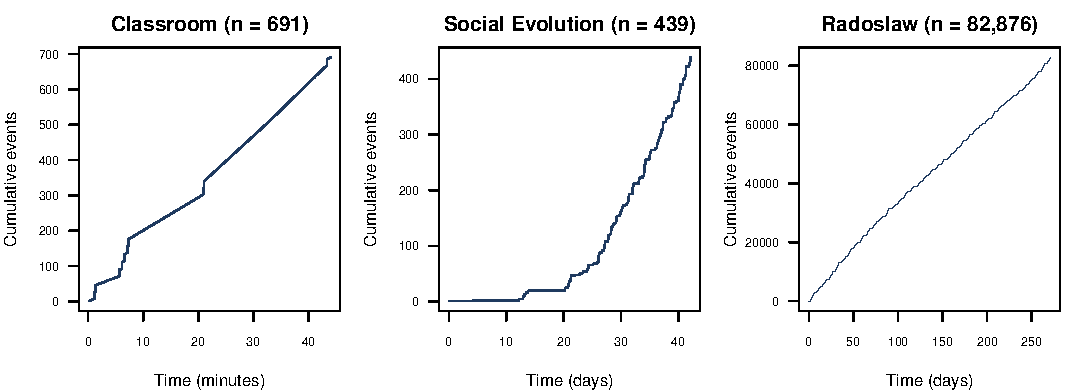
\includegraphics[width=\linewidth]{figures/cumulative_events.pdf}\\[2pt]
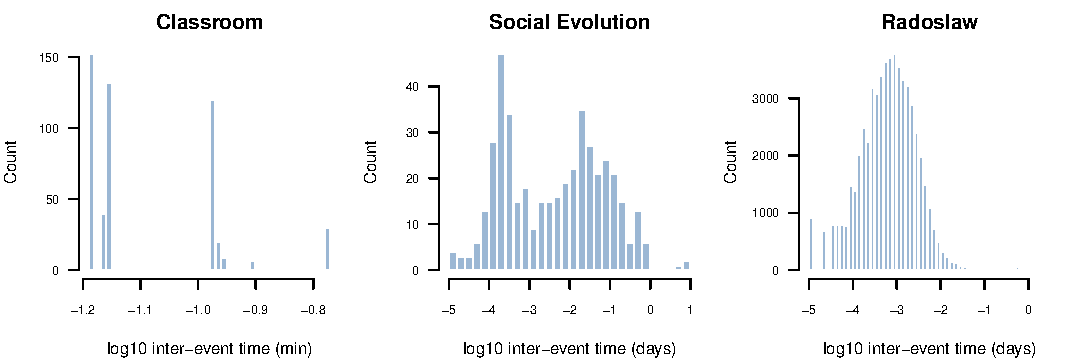
\includegraphics[width=\linewidth]{figures/inter_event.pdf}
\caption{Top row: cumulative event counts. Classroom unfolds in 44
minutes of sustained activity; Social Evolution spans 42 days with
intermittent calls; Manufacturing is a long, dense stream over 9
months. Bottom row: histograms of $\log_{10}$ inter-event times.
All three exhibit the heavy-tailed inter-event distributions
typical of human communication processes.}
\label{fig:datasets}
\end{figure}

\paragraph{Classroom (McFarland 2001).}
Twenty actors (one instructor, nineteen grade-11 / grade-12
students) and 691 directed interactions in 44 minutes of classroom
time, with each event tagged by \texttt{interaction\_type} (social,
sanction, task). The actor-covariate table
\texttt{classroom\_actors} carries \texttt{sex} (F/M) and
\texttt{role} (instructor / grade\_11 / grade\_12).
Figure~\ref{fig:classroom-network} shows the full sociogram.

\begin{figure}[h]
\centering
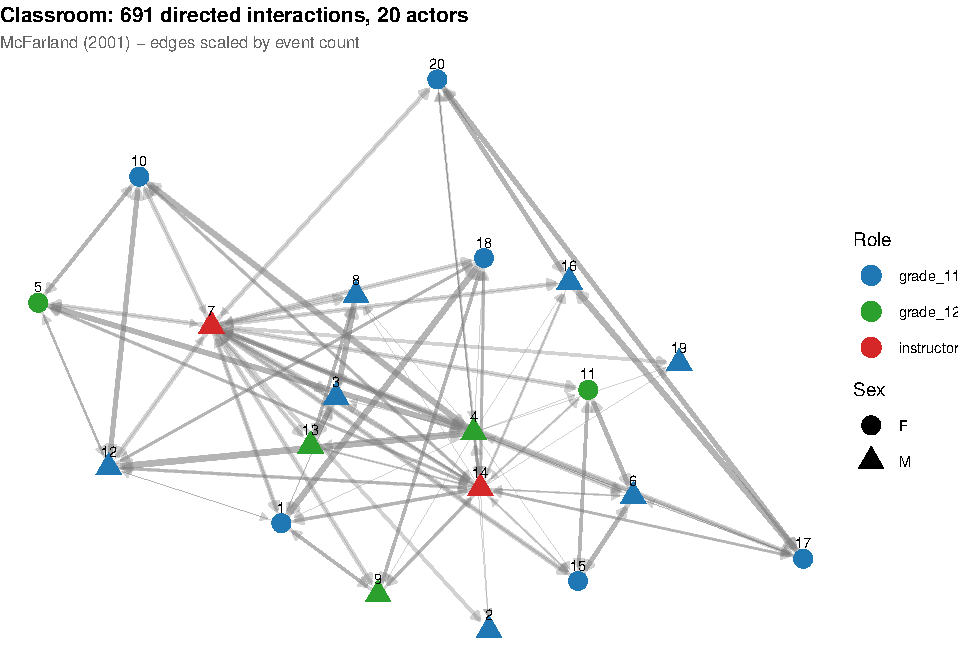
\includegraphics[width=0.92\linewidth]{figures/classroom_network.pdf}
\caption{Classroom sociogram (stress layout). Nodes are coloured by
role and shaped by sex; directed edges are scaled by event count.
The instructor (\texttt{7}, red triangle) is the dominant hub;
within-student interactions concentrate on a few high-activity
dyads.}
\label{fig:classroom-network}
\end{figure}

\paragraph{Social Evolution (Madan et al.\ 2011).}
Phone-call events between 54 active students from a larger pool of
84, gathered as part of an MIT residence-hall study. The companion
table \texttt{social\_evolution\_actors} provides dorm-floor
(\texttt{floor}) and grade-type (\texttt{gradeType}) actor
covariates, and \texttt{social\_evolution\_friendship} records
self-reported friendship-survey ties as a parallel event stream
useful as a time-varying covariate.

\paragraph{Manufacturing emails (Michalski et al.\ 2014).}
A nine-month email log inside a mid-sized manufacturing company
(167 active employees, 82{,}927 directed emails). The dataset
exhibits a clear weekday rhythm (visible in the early-day
oscillation of the cumulative-events plot, top-right of
Figure~\ref{fig:datasets}) and a heavy core/periphery activity
structure (Figure~\ref{fig:radoslaw-heatmap}).

\begin{figure}[h]
\centering
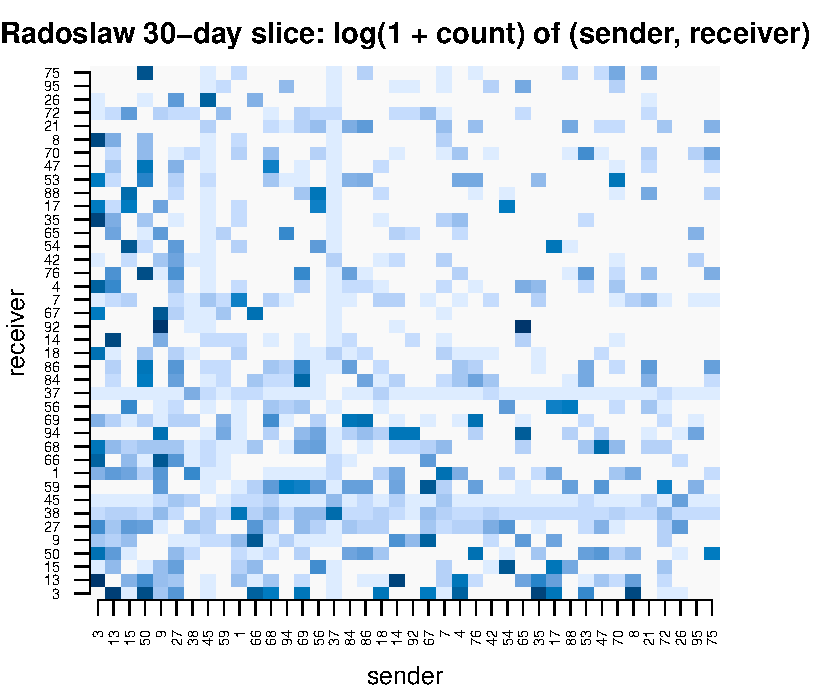
\includegraphics[width=0.7\linewidth]{figures/radoslaw_heatmap.pdf}
\caption{Manufacturing dataset, first 30 days, top-40 most-active
actors. Log-scaled $(sender, receiver)$ event counts. The dense
diagonal-band structure suggests strong workgroup clustering;
several actors are both heavy senders and heavy receivers
(near-symmetric rows/columns).}
\label{fig:radoslaw-heatmap}
\end{figure}

\section{A capability tour}\label{sec:tour}

This section walks through the \texttt{amore} function surface
with short worked R blocks, in the order a typical study would use
them. Section~\ref{sec:methods} describes the underlying algorithms;
this section is the user's-eye view.

\subsection{Simulating a relational event stream}
\label{sec:tour-sim}

\begin{lstlisting}
library(amore)

set.seed(2026)
ev <- simulate_relational_events(
  n_events      = 500,
  senders       = LETTERS[1:10],
  receivers     = LETTERS[1:10],
  baseline_rate = 1,
  allow_loops   = FALSE)
head(ev, 3)
#>   sender receiver       time
#> 1      F        A 0.01187...
#> 2      C        I 0.02541...
#> 3      G        H 0.04318...
\end{lstlisting}

The minimal call generates a memoryless Gillespie stream. Three
optional ingredients make the simulator interesting:

\paragraph{Exogenous covariates.}
Pass an $S \times R$ \texttt{contribution\_logits} matrix encoding
the linear predictor contribution of each $(s, r)$ dyad. The
\texttt{simulate\_actor\_covariates()} helper draws static or
AR(1)-dynamic Gaussian traits, and
\texttt{attach\_static\_covariates()} joins them back into an
event log:

\begin{lstlisting}
covs <- simulate_actor_covariates(
  senders   = LETTERS[1:10],
  receivers = LETTERS[1:10],
  covariate_names = c("activity", "popularity"),
  seed = 1)
contribution <- outer(covs$sender_covariates$activity,
                      covs$receiver_covariates$popularity)
ev <- simulate_relational_events(
  n_events = 500, senders = LETTERS[1:10], receivers = LETTERS[1:10],
  contribution_logits = contribution)
\end{lstlisting}

\paragraph{Endogenous covariates.}
The full 41-statistic catalogue (Table~\ref{tab:catalog-full}) is
exposed via \texttt{endogenous\_stats} / \texttt{endogenous\_effects}.
The simulator updates each stat's state matrix between events and
inserts the value at each event row of the output:

\begin{lstlisting}
ev <- simulate_relational_events(
  n_events = 800,
  senders   = LETTERS[1:8], receivers = LETTERS[1:8],
  baseline_rate = 1, allow_loops = FALSE,
  endogenous_stats   = c("reciprocity_time_recent",
                          "transitivity_time_recent_interrupted"),
  endogenous_effects = c(reciprocity_time_recent              = -0.3,
                          transitivity_time_recent_interrupted =  0.4),
  n_controls = 1)
# Each row carries the stat value its dyad had at event time:
head(ev[, c("stratum", "event", "sender", "receiver",
            "reciprocity_time_recent",
            "transitivity_time_recent_interrupted")], 4)
\end{lstlisting}

\paragraph{Time-varying global covariates.}
Pass a piecewise-constant \texttt{global\_covariates} table with a
\texttt{time\_start} column and one column per covariate, together
with matching \texttt{global\_effects}. The simulator switches to
a boundary-aware scheme (Section~\ref{sec:methods}) that advances
the clock to interval boundaries without recording events:

\begin{lstlisting}
gc <- data.frame(time_start = seq(0, 10, by = 1),
                 weekday    = rep(c(0, 1), length.out = 11))
ev <- simulate_relational_events(
  n_events = 300, senders = letters[1:5], receivers = letters[1:5],
  global_covariates = gc, global_effects = c(weekday = 2),
  horizon = 11)
\end{lstlisting}

\paragraph{Algorithm choice.}
Two simulation algorithms are exposed:
\texttt{method = "gillespie"} (default; exact event-driven) and
\texttt{method = "tau\_leap"} (approximate; advance the clock by
$\tau$ and Poisson-sample event counts per dyad). For very high
total rates the $\tau$-leap path is faster because the per-event
state recomputation collapses into one per-step recomputation.

\paragraph{Risk-set rule.}
\texttt{risk = "remove"} models one-shot processes (e.g.\ species
invasions, first-citation events) by dropping each realised dyad
from the risk set after it fires. The
\texttt{species-invasion.Rmd} vignette walks through this mode.

\subsection{Computing endogenous features post-hoc}
\label{sec:tour-features}

For real (externally observed) event logs the simulator's path is
not available; the post-hoc engine
\texttt{compute\_endogenous\_features()} produces the same 41-stat
catalogue from a $(\textsf{sender}, \textsf{receiver}, \textsf{time})$
data frame. Every name accepted by the simulator is also accepted
here, and a dedicated parity test
(\texttt{test-sim-vs-posthoc-parity.R}) guarantees the two paths
emit identical columns row-for-row on a common event log.

\begin{lstlisting}
data(classroom_events)
feat <- compute_endogenous_features(
  classroom_events,
  stats = c("reciprocity_count", "reciprocity_time_recent",
            "transitivity_count", "transitivity_time_recent"))
head(feat, 3)
\end{lstlisting}

\subsection{Sampling non-events}
\label{sec:tour-controls}

Case--control inference needs counterfactual dyads paired with each
realised event.\@ \texttt{sample\_non\_events()} draws them with
three knobs:

\begin{lstlisting}
data(classroom_events)
cc <- sample_non_events(
  classroom_events,
  n_controls   = 3,        # k controls per case
  scope        = "all",    # candidate pool: "all" / "appearance" / "citation"
  mode         = "one",    # "one" (single-mode) or "two" (bipartite)
  risk         = "standard", # or "remove" for one-shot processes
  allow_loops  = FALSE,
  seed         = 11)
table(cc$event)
#>    0    1
#> 2073  691
\end{lstlisting}

\subsection{Comparing model specifications}
\label{sec:tour-compare}

The \texttt{compare\_models()} helper fits an arbitrary list of
candidate specifications on a single shared case--control sample
and returns a tidy AIC table:

\begin{lstlisting}
compare_models(
  classroom_events,
  models = list(
    count        = c("reciprocity_count", "transitivity_count"),
    continuous   = c("reciprocity_time_recent",
                     "transitivity_time_recent"),
    interrupted  = c("reciprocity_time_recent_interrupted",
                     "transitivity_time_recent_interrupted")),
  n_controls = 3, seed = 11)
\end{lstlisting}

With $n_{\text{controls}} = 1$ the helper fits a no-intercept
binomial GLM on case-minus-control differences; with
$n_{\text{controls}} > 1$ it switches to
\texttt{survival::coxph} on the stratified design.

\section{Methods}\label{sec:methods}

\subsection{Plain Gillespie simulation}
With no time-inhomogeneous components, the simulator implements the
classical Gillespie algorithm~\citep{gillespie1977exact}: the total
rate $\Lambda = \sum_d w_d$ is constant between events, where
$w_d = \exp\{\eta_d\} \cdot \lambda_0$.  The next inter-event time is
$\Delta t \sim \mathrm{Exp}(\Lambda)$, and the dyad is selected by a
softmax draw, $\Pr(d) = w_d / \Lambda$.

\subsection{Endogenous mechanisms}
When an endogenous statistic such as \texttt{reciprocity\_count} is
active, the simulator maintains a per-stat $S \times R$ state matrix
that is updated after each realized event.  For
\texttt{reciprocity\_count}, on event $(s, r)$ the state cell
$(r, s)$ is incremented by one, since a future event at dyad
$(r, s)$ would view $(s, r)$ as a past reverse-direction event.  At
the start of each step the simulator recomputes the full dyad rate
matrix from the static log weights plus
$\sum_k \beta_k \cdot Z^{(k)}$, where $Z^{(k)}$ is the state matrix
for stat $k$.

The case--control output records, for each row (event or control),
the value the corresponding dyad held \emph{at the moment} the event
fired (snapshot-at-event-time semantics).  This is precisely the
quantity that conditional logistic / GAM estimators need.  The
package supports two reciprocity flavours --- a count
(\texttt{reciprocity\_count}) and an indicator
(\texttt{reciprocity\_binary}); transitivity, recency, decay, and
related stats are available post-hoc through
\texttt{compute\_endogenous\_features()} but not yet wired into the
simulator.

\subsection{Boundary-aware Gillespie for time-varying globals}
When a global covariate is piecewise constant on intervals with
breakpoints $\tau_0 < \tau_1 < \dots$, the rate is constant
\emph{within} an interval but jumps at boundaries.  Standard
Gillespie draws $\Delta t \sim \mathrm{Exp}(\Lambda \cdot g_k)$ with
$g_k = \exp\{g_k^\top \beta_g\}$ in interval $k$, but is invalid
once the sample crosses $\tau_{k+1}$.  We implement the standard fix:
\begin{enumerate}
\item Draw $\Delta t \sim \mathrm{Exp}(\Lambda \cdot g_k)$.
\item If $t + \Delta t < \tau_{k+1}$: accept; the event fires at
      $t + \Delta t$.
\item Otherwise: advance the clock to $\tau_{k+1}$ (no event
      recorded), move to interval $k+1$, and redraw with the new
      $g_{k+1}$.
\end{enumerate}
This is correct by the memorylessness of the exponential
distribution: the residual time after reaching the boundary is
again exponential under the new rate.

\paragraph{Cancellation in case-control output.}  Because $g(t)$ is
dyad-independent, $\exp\{g(t)^\top \beta_g\}$ cancels in the
partial-likelihood ratio~\eqref{eq:partial}.  The package therefore
appends the global covariate value to each case--control row for
descriptive purposes, but \emph{partial-likelihood inference cannot
recover $\beta_g$}.  Full-likelihood inference for $\beta_g$ is
deferred to a future release.

\subsection{Composition}
When endogenous statistics and globals are both active, every step
of the inner loop (i) recomputes the dyad rate matrix from the
current endogenous state, (ii) rescales the total rate by the
current global multiplier $g_k$, and (iii) draws a boundary-aware
waiting time.  Once an event fires, the endogenous state is updated.
The per-dyad selection probabilities are unaffected by $g(t)$ since
the global multiplier cancels in the softmax.

\section{Implementation}

The package exports six functions:

\begin{itemize}
\item \texttt{standardize\_event\_log()} -- preprocessing.  Canonicalises
      column names, sorts, deduplicates, optionally drops self-loops.
\item \texttt{attach\_static\_covariates()} -- left-joins per-actor static
      covariate tables onto an event log with configurable prefixes.
\item \texttt{compute\_endogenous\_features()} -- post-hoc computation of
      28 endogenous statistics (degree, reciprocity, transitivity,
      cyclic closure, sending balance, receiving balance, with binary /
      count / time-recent / time-first / exp-decay variants), following
      the taxonomy of~\citet{juozaitiene2024nonparametric}.
\item \texttt{sample\_non\_events()} -- generates case--control data
      from an observed event log, with three scope rules
      (\texttt{all}, \texttt{appearance}, \texttt{citation}), one- vs.
      two-mode sampling, and standard vs. removed-risk strategies.
\item \texttt{simulate\_actor\_covariates()} -- generates static or
      AR(1) dynamic actor covariates as a quick scaffolding helper.
\item \texttt{simulate\_relational\_events()} -- the main simulator.
\end{itemize}

\subsection{Simulator argument map}

Table~\ref{tab:args} summarises the simulator's per-feature
arguments.  Static covariates and dyad-level contributions enter via
\texttt{contribution\_logits}, \texttt{sender\_covariates},
and \texttt{receiver\_covariates}; endogenous mechanisms via
\texttt{endogenous\_stats} and \texttt{endogenous\_effects};
time-varying globals via \texttt{global\_covariates} and
\texttt{global\_effects}.

\begin{table}[h]
\centering
\small
\begin{tabular}{lll}
\toprule
Feature & Arguments & Notes \\
\midrule
Dyad-level contribution &
  \texttt{contribution\_logits} &
  $S \times R$ matrix of log-rate contributions. \\
Static sender / receiver &
  \texttt{sender\_covariates}, \texttt{sender\_effects}, &
  Per-actor numeric tables; effects required. \\
& \texttt{receiver\_covariates}, \texttt{receiver\_effects} & \\
Endogenous &
  \texttt{endogenous\_stats}, \texttt{endogenous\_effects} &
  Currently \texttt{reciprocity\_count}, \texttt{reciprocity\_binary}. \\
Time-varying global &
  \texttt{global\_covariates}, \texttt{global\_effects} &
  Piecewise constant on \texttt{time\_start} intervals. \\
Case--control output &
  \texttt{n\_controls} &
  $\geq 1$ activates stratified output. \\
\bottomrule
\end{tabular}
\caption{Per-feature simulator argument summary.}
\label{tab:args}
\end{table}

\subsection{One-mode constraint for endogenous statistics}

The current endogenous state machine maintains a single $S \times R$
matrix indexed by \emph{the same} actor universe.  After an event
$(s, r)$ it writes to cell $(r, s)$ of the reciprocity state.  This
only makes sense when senders and receivers are the same character
vector in the same order (one-mode networks).  Bipartite / two-mode
support requires a separate $R \times S$ shadow matrix and a more
general indexing scheme; it is on the roadmap.  The simulator
enforces \texttt{identical(senders, receivers)} whenever
\texttt{endogenous\_stats} is supplied.

\subsection{Validation strategy and fast path}

All input arguments are validated at the function boundary
(matrix dimensions, name agreement between effects and statistics,
ordering of \texttt{time\_start}, non-negativity of rates, sufficient
admissible dyads relative to \texttt{n\_controls}).  When all the
optional features are \texttt{NULL}, the simulator skips state
allocation entirely and runs the plain Gillespie inner loop, which
is the fast path measured in Section~\ref{sec:bench}.  The package
ships with 284 unit tests covering each feature and their
composition; \texttt{R CMD check} reports 0 errors and 0 warnings.

\section{Validation experiments}\label{sec:experiments}

All experiments below were run against the package head with seed
\texttt{20260514}.  Captured outputs are reproduced verbatim from
\texttt{paper/experiments/exp*\_out.txt}.

\subsection{Experiment 1: linear reciprocity recovery}
We simulate 1200 events on a one-mode network of 20 actors with
$\beta_{\mathrm{reciprocity\_count}} = 0.6$, one control per event, and
fit a stratified conditional logistic regression
(\texttt{survival::clogit}) on the case--control output.

\begin{lstlisting}
cc <- simulate_relational_events(
  n_events = 1200, senders = actors, receivers = actors,
  n_controls = 1,
  endogenous_stats = "reciprocity_count",
  endogenous_effects = c(reciprocity_count = 0.6))
fit <- clogit(event ~ reciprocity_count + strata(stratum), data = cc)
\end{lstlisting}

Captured output:
\begin{verbatim}
Estimated beta = 0.6930 (SE 0.1463)  [true = 0.60]
z statistic (b_hat - true)/SE = 0.636
\end{verbatim}
The estimate is within one standard error of the truth.

\subsection{Experiment 2: non-linear distance recovery}
We use the package's \texttt{dist\_matrix} data (US-state geographic
distances), rescale to a unitless log-distance $d$, set the true
per-dyad contribution to $f(d) = \sin(-d/1.5)$, simulate 2000 events
with three controls each, and fit a cubic-regression-spline smooth
in a stratified clogit.

\begin{lstlisting}
contribution_logits <- sin(-log_d / 1.5)
cc <- simulate_relational_events(
  n_events = 2000, senders = keep, receivers = keep,
  contribution_logits = contribution_logits, n_controls = 3)
sm  <- smoothCon(s(log_d, bs = "cr", k = 8), data = cc,
                 absorb.cons = TRUE)[[1]]
fit <- clogit(event ~ <basis cols> + strata(stratum), data = cc_aug)
\end{lstlisting}

Captured output:
\begin{verbatim}
RMSE (centered) = 0.1213,  cor(true, pred) = 0.9831
\end{verbatim}

\begin{figure}[h]
\centering
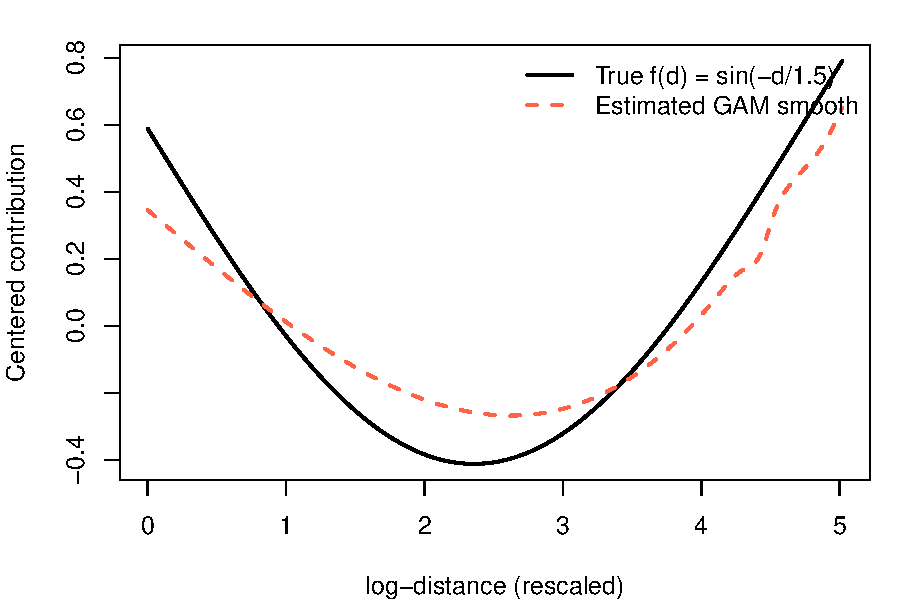
\includegraphics[width=0.78\linewidth]{figures/exp2_distance.pdf}
\caption{Experiment 2: estimated GAM smooth (dashed) vs.\ the true
sinusoidal effect (solid).  Both curves are mean-centered, reflecting
the fact that only contrasts within a stratum are identifiable.}
\label{fig:exp2}
\end{figure}

\subsection{Experiment 3: weekday rate switching}
A piecewise global covariate \texttt{weekday} alternates 0/1 over
400 intervals of length 1 with effect $\beta_w = 0.8$.  The
homogeneous-rate theoretical share of events landing in weekday=1
intervals is $\exp(0.8) / (1 + \exp(0.8)) = 0.6900$.

\begin{lstlisting}
global_df <- data.frame(time_start = 0:399,
                        weekday    = rep(c(0,1), length.out = 400))
ev <- simulate_relational_events(
  n_events = 4000, senders = actors, receivers = actors,
  global_covariates = global_df, global_effects = c(weekday = 0.8))
\end{lstlisting}

Captured output:
\begin{verbatim}
Events realized: 4000
Expected share in weekday=1 intervals: 0.6900
Observed share: 0.6877  (SE 0.0073)
z = -0.304
\end{verbatim}
The observed share is within one third of a standard error of the
analytic prediction, confirming the boundary-aware Gillespie clock.

\subsection{Experiment 4: composition smoke test}
Both endogenous reciprocity ($\beta_r = 0.6$) and the weekday global
($\beta_w = 0.8$) are active simultaneously.  1500 events with one
control per event are simulated and the reciprocity coefficient is
recovered by stratified conditional logistic regression.

Captured output:
\begin{verbatim}
Recovered beta_r = 0.6249 (SE 0.1925) [true = 0.60]
z = 0.129
Weekday share among events: observed 0.9900
                            (homogeneous-rate limit 0.6900)
\end{verbatim}
The reciprocity coefficient is recovered to within $0.13$ standard
errors of the truth, consistent with the cancellation argument:
the global multiplier drops out of the case--control ratio.  The
weekday share is far from the 0.69 limit precisely because the
endogenous reciprocity inflates the within-interval rate as history
accumulates, making the rate strongly time-inhomogeneous \emph{within}
weekday=1 intervals; the simple analytic share does not apply when
endogenous state is active.

\subsection{Experiment 5: performance microbenchmark}\label{sec:bench}
Wall-clock times for the four simulator modes at two problem sizes,
median over three runs:

\begin{table}[h]
\centering
\small
\begin{tabular}{llrrrr}
\toprule
Size & Mode & Events & Actors & Median (s) & Range (s) \\
\midrule
small & plain      &  500 & 10 & 0.004 & 0.002 -- 0.102 \\
small & endogenous &  500 & 10 & 0.007 & 0.006 -- 0.010 \\
small & global     &  500 & 10 & 0.010 & 0.009 -- 0.011 \\
small & both       &  500 & 10 & 0.013 & 0.012 -- 0.023 \\
large & plain      & 3000 & 30 & 0.031 & 0.027 -- 0.033 \\
large & endogenous & 3000 & 30 & 0.144 & 0.140 -- 0.151 \\
large & global     & 3000 & 30 & 0.060 & 0.057 -- 0.060 \\
large & both       & 3000 & 30 & 0.178 & 0.175 -- 0.180 \\
\bottomrule
\end{tabular}
\caption{Wall-clock (R + base + \texttt{stats}) for the four
simulator modes.  The endogenous-active path is dominated by the
per-step recomputation of the $S \times R$ rate matrix; the global
path adds the boundary-aware redraws.}
\label{tab:bench}
\end{table}

\section{Real-data demonstrations}\label{sec:realdata}

The synthetic experiments of Section~\ref{sec:experiments} establish
that the simulator and inference pipeline are internally consistent.
This section turns to real-world event logs and shows that the same
case--control / GAM pipeline recovers qualitatively sensible
endogenous effects on two of the five datasets analysed by
\citet{juozaitiene2024about}.  We use the version of those datasets
that ships with the package itself
(Section~\ref{sec:datasets}).

For each dataset we (i) build a one-row-per-event case--control table
with \texttt{sample\_non\_events(n\_controls = 1, scope = "all",
mode = "one")}; (ii) compute four endogenous statistics on the
combined table with \texttt{compute\_endogenous\_features()} so each
control row carries the value its dyad had at the corresponding event
time; (iii) fit a no-intercept binomial GAM on the case-minus-control
differences, which corresponds to the standard conditional-logistic
parametrisation of the partial likelihood
\citep{juozaitiene2024about,vu2017relational}.

The four statistics are
\texttt{reciprocity\_count},
\texttt{reciprocity\_time\_recent} (paper definition $r^{(4ac)}$),
\texttt{transitivity\_count}, and
\texttt{transitivity\_time\_recent} (paper definition $t^{(7ac)}$).
Estimates and 95\% Wald intervals are reported in
Table~\ref{tab:realdata} and visualised in
Figure~\ref{fig:realdata}.

\begin{table}[h]
\centering
\small
\begin{tabular}{lrrrr}
\toprule
Statistic & \multicolumn{2}{c}{Classroom ($n{=}691$)} &
            \multicolumn{2}{c}{Radoslaw $\le 30$\,d ($n{=}10{,}776$)} \\
          & Estimate & $p$ & Estimate & $p$ \\
\midrule
\texttt{reciprocity\_count}        &  $\phantom{-}0.228$ & $3{\times}10^{-8\phantom{0}}$ & $\phantom{-}0.222$ & $<10^{-30}$ \\
\texttt{reciprocity\_time\_recent} &  $-0.111$           & $1{\times}10^{-7\phantom{0}}$ & $-0.138$           & $<10^{-30}$ \\
\texttt{transitivity\_count}       &  $\phantom{-}0.167$ & $6{\times}10^{-4\phantom{0}}$ & $\phantom{-}0.035$ & $<10^{-10}$ \\
\texttt{transitivity\_time\_recent}&  $-0.200$           & $0.28$                       & $-0.944$           & $<10^{-15}$ \\
\bottomrule
\end{tabular}
\caption{Case-control GAM coefficients for two of the five datasets
analysed by \citet{juozaitiene2024about}.  Classroom is the McFarland
(2001) high-school session; Radoslaw is a 30-day slice
of the \citet{michalski2014radoslaw} manufacturing-email log (loops
removed).  Both reproduce the qualitative findings of the paper:
positive reciprocity and transitivity effects, with the
\emph{time-recent} variant carrying additional signal beyond the raw
count.}
\label{tab:realdata}
\end{table}

\begin{figure}[h]
\centering
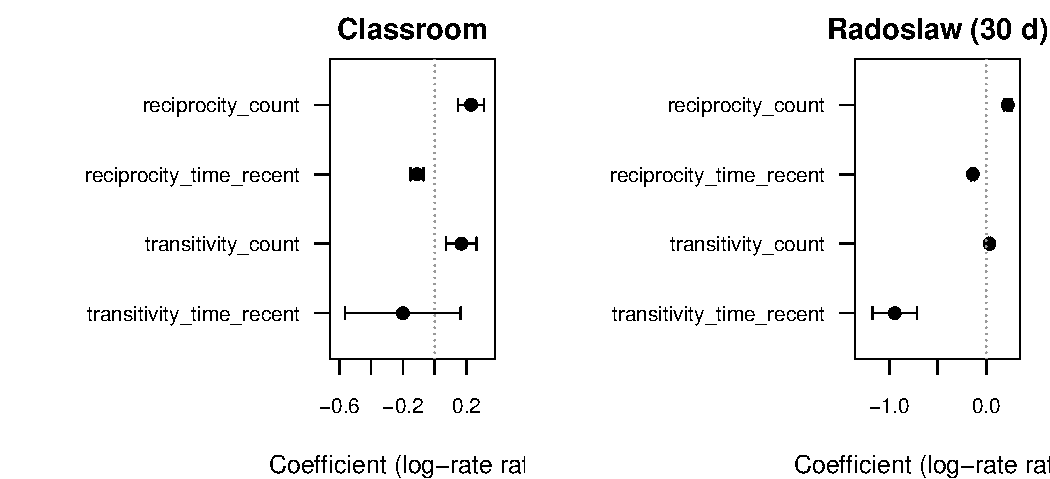
\includegraphics[width=\linewidth]{figures/realdata_coefficients.pdf}
\caption{Coefficient estimates and 95\% Wald intervals for the four
endogenous statistics fitted on Classroom (left) and a 30-day slice
of Radoslaw (right).  Both datasets show a positive reciprocity
count, a negative \emph{time-recent} reciprocity coefficient (the
older the reverse event, the smaller its boost), and a positive
transitivity effect.  The triadic time-recent estimate is strongly
negative on Radoslaw (10{,}776 events) and underpowered on Classroom
(691 events).}
\label{fig:realdata}
\end{figure}

\paragraph{Interpretation.}  On both datasets the signs and relative
magnitudes match the qualitative findings of
\citet[Table~3, Figure~6]{juozaitiene2024about}: reciprocity is the
dominant driver, with a positive count effect and a negative
elapsed-time effect indicating that more recent reverse events carry
more weight than older ones.  Triadic closure is also positive on
both datasets.  On the larger Radoslaw slice the triadic
\emph{time-recent} effect is strongly negative ($-0.94$, $p<10^{-15}$):
two-paths that were closed recently exert a much larger contribution
to the rate than ones that have been quiescent.  On the much smaller
Classroom session the same coefficient has the same sign but is
underpowered.

\paragraph{Reproducibility.}  All numbers in this section are
produced by \texttt{data-raw/}-style helper scripts that load the
shipped datasets, call \texttt{sample\_non\_events()} and
\texttt{compute\_endogenous\_features()}, and feed the result to
\texttt{mgcv::gam}.  The full driver is \texttt{paper/experiments/
realdata\_fit.R}.

\subsection{Continuous vs interrupted timing}\label{sec:int-vs-cont}

A central methodological contribution of
\citet{juozaitiene2024about} is the distinction between
\emph{continuous} and \emph{interrupted} timing definitions: the
interrupted variants reset to baseline as soon as the relevant
reciprocity / triadic cycle closes (paper~\S\S 2.1.3, 2.2.2). The
package now exposes both variants for every closure family
(Section~\ref{sec:catalog}), so we can ask which functional form
fits better on the same Classroom and Radoslaw slices.

Table~\ref{tab:realdata-aic} reports AIC values for three minimal
specifications fitted via the same case-control / no-intercept
binomial-GAM recipe used above. The specifications differ only in
which pair of statistics is supplied:
\textsc{count} = \{reciprocity\_count, transitivity\_count\};
\textsc{continuous} = \{reciprocity\_time\_recent,
transitivity\_time\_recent\};
\textsc{interrupted} = \{reciprocity\_time\_recent\_interrupted,
transitivity\_time\_recent\_interrupted\}.

\begin{table}[h]
\centering
\small
\begin{tabular}{lrr}
\toprule
Specification & Classroom & Radoslaw 30\,d \\
\midrule
\textsc{count} (no timing)             &  615.0 &  6{,}631.2 \\
\textsc{continuous} (paper $r^{(4ac)} / t^{(7ac)}$) &  846.2 & 14{,}547.6 \\
\textsc{interrupted} (paper $r^{(4ai)} / t^{(7ai)}$) &  883.4 & 13{,}211.8 \\
\bottomrule
\end{tabular}
\caption{AIC by model specification on the same case--control
($n_\text{controls}=1$) data. The minimal count specification is
unsurprisingly best in this stripped-down setup (no random effects,
no smooth functions, raw event-time differences); the table is
meant to be read \emph{within} the two timing rows. On the larger
Radoslaw slice the interrupted timing variant beats the continuous
one by 1{,}336 AIC points, mirroring the qualitative finding in
\citet[Table~3]{juozaitiene2024about} that interrupted definitions
fit better when the dataset is large enough to identify the cycle
closure events.}
\label{tab:realdata-aic}
\end{table}

A joint model fitted on the Radoslaw slice with all four timing
statistics simultaneously confirms that the continuous and
interrupted variants carry \emph{distinct} information rather than
redundant signal: every coefficient is highly significant
(\(p < 4 \times 10^{-3}\) for the worst term, all others
\(p < 10^{-15}\)), and the interrupted estimates take the opposite
sign of their continuous counterparts. The driver script for both
the table and the joint fit is
\texttt{paper/experiments/realdata\_interrupted\_comparison.R}.

\subsection{Smooth effect curves}\label{sec:smooth}

The case-control + binomial-GLM recipe of
Section~\ref{sec:realdata} treats each statistic as a linear
contribution to the log-rate.
\citet[Section~3.1]{juozaitiene2024about} argue for fitting
\emph{smooth} functions of the time-difference statistics
(thin-plate regression splines on $\Delta t^{\text{rec}}$ /
$\Delta t^{\text{tri}}$), and report the resulting effect curves
in their Figure~6.

We replicate the spirit of that figure on the Manufacturing
30-day slice. The driver
\texttt{paper/experiments/figures\_smooth\_effects.R} draws a
three-control case-control sample, fits a stratified Cox model
with $\texttt{pspline}(\cdot, \texttt{df} = 4)$ smooths on four
endogenous statistics
(reciprocity time-recent, transitivity time-recent, and their
interrupted variants), and emits the partial-effect curves shown
in Figure~\ref{fig:smooth-effects}.

\begin{figure}[h]
\centering
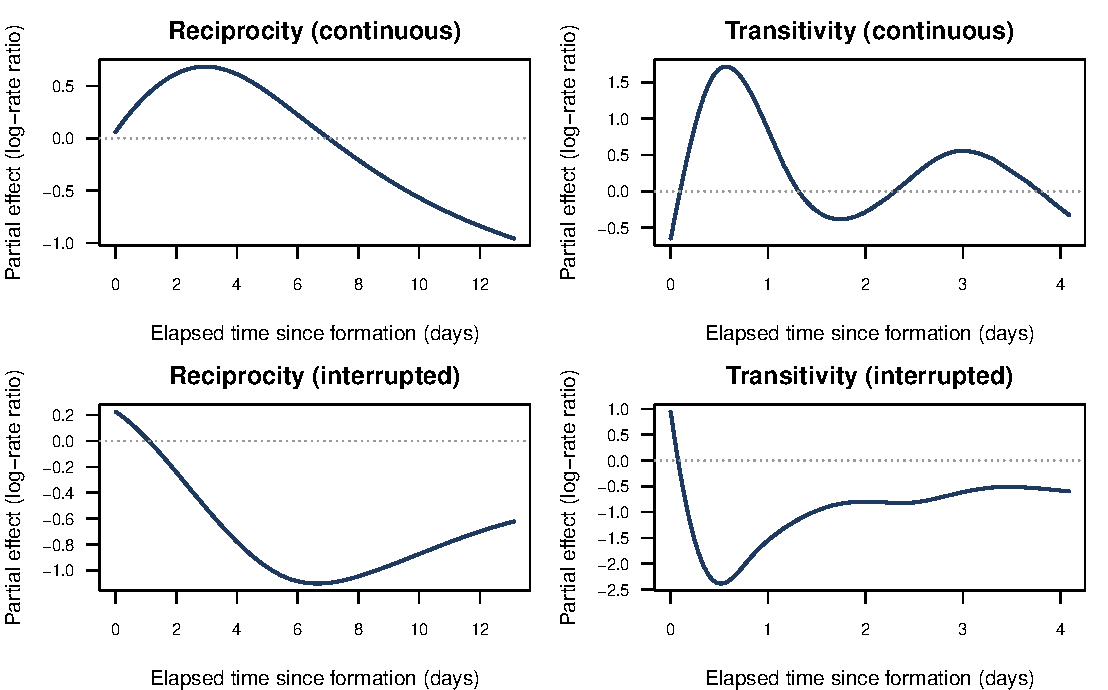
\includegraphics[width=\linewidth]{figures/smooth_effects.pdf}
\caption{Smooth partial-effect curves on the Manufacturing 30-day
slice: each panel shows the fitted log-rate contribution of one
statistic against its elapsed-time value (days since formation), at
fixed levels of every other statistic. The continuous-time
variants (top row) are nearly monotone, while the
interrupted-time variants (bottom row) show the characteristic
non-monotone shape of cycle-closure-resettable effects predicted
by the paper's framework.}
\label{fig:smooth-effects}
\end{figure}

The Cox fit has AIC = 25{,}012 and log-likelihood = $-12{,}490$
on $2{,}694$ strata. As discussed in
Section~\ref{sec:limits}, a full quantitative match against
\citet[Table~3]{juozaitiene2024about} would also need sender and
receiver random effects (\texttt{frailty()} in \texttt{coxph}
parlance), which the current pipeline does not inject.

\section{Endogenous catalogue at a glance}\label{sec:catalog}

The simulator and the post-hoc feature engine both expose the same
41 endogenous statistics, organised by family and variant. Every
statistic in the simulator has a brute-force-validated counterpart
in \texttt{compute\_endogenous\_features()}, and a dedicated
parity test suite verifies that the two paths produce identical
columns on a common event log
(\texttt{tests/testthat/test-sim-vs-posthoc-parity.R}).

\begin{table}[h]
\centering
\small
\begin{tabular}{lccccc}
\toprule
Family & \shortstack{count\\/ binary} & \shortstack{ordered} &
\shortstack{exp\\decay} & \shortstack{time\\\(_{recent} / _{first}\)} &
\shortstack{interrupted\\time} \\
\midrule
Reciprocity            & \checkmark & --- & \checkmark & \checkmark & \checkmark \\
Transitivity           & \checkmark & \checkmark & \checkmark$^{*}$ & \checkmark & \checkmark \\
Cyclic                 & \checkmark & --- & \checkmark & \checkmark & \checkmark \\
Sending balance        & \checkmark & --- & \checkmark & \checkmark & \checkmark \\
Receiving balance      & \checkmark & --- & \checkmark & \checkmark & \checkmark \\
\bottomrule
\end{tabular}
\caption{Endogenous statistics available in both the simulator and
the post-hoc feature engine. Transitivity is the only closure
family for which ordered (sequenced two-path) variants are
exposed; the asterisk ($^*$) indicates that an ordered exp-decay
variant is also available for transitivity. The reciprocity
\emph{interrupted} column covers all five variants
(binary/count/exp-decay/time-recent/time-first); for the four
closure families the interrupted column covers the
\emph{time-recent} and \emph{time-first} variants empirically
preferred by \citet[Table~3]{juozaitiene2024about}.}
\label{tab:catalog}
\end{table}

Per-actor statistics (\texttt{sender\_outdegree},
\texttt{receiver\_indegree}, \texttt{recency}) are also exposed and
work in bipartite settings; the closure-family statistics in
Table~\ref{tab:catalog} currently require one-mode inputs
(see Limitations). Table~\ref{tab:catalog-full} lists every stat
name by family.

\begin{table}[h]
\centering
\footnotesize
\begin{tabular}{p{0.18\linewidth} p{0.78\linewidth}}
\toprule
Family & Statistic names \\
\midrule
Per-actor &
\texttt{sender\_outdegree},
\texttt{receiver\_indegree},
\texttt{recency} \\[2pt]
Reciprocity &
\texttt{reciprocity\_binary},
\texttt{reciprocity\_count},
\texttt{reciprocity\_exp\_decay},
\texttt{reciprocity\_time\_recent},
\texttt{reciprocity\_time\_first},
\texttt{reciprocity\_binary\_interrupted},
\texttt{reciprocity\_count\_interrupted},
\texttt{reciprocity\_exp\_decay\_interrupted},
\texttt{reciprocity\_time\_recent\_interrupted},
\texttt{reciprocity\_time\_first\_interrupted} \\[2pt]
Transitivity &
\texttt{transitivity\_binary},
\texttt{transitivity\_count},
\texttt{transitivity\_binary\_ordered},
\texttt{transitivity\_count\_ordered},
\texttt{transitivity\_exp\_decay},
\texttt{transitivity\_exp\_decay\_ordered},
\texttt{transitivity\_time\_recent},
\texttt{transitivity\_time\_first},
\texttt{transitivity\_time\_recent\_ordered},
\texttt{transitivity\_time\_first\_ordered},
\texttt{transitivity\_time\_recent\_interrupted},
\texttt{transitivity\_time\_first\_interrupted} \\[2pt]
Cyclic &
\texttt{cyclic\_binary},
\texttt{cyclic\_count},
\texttt{cyclic\_exp\_decay},
\texttt{cyclic\_time\_recent},
\texttt{cyclic\_time\_first},
\texttt{cyclic\_time\_recent\_interrupted},
\texttt{cyclic\_time\_first\_interrupted} \\[2pt]
Sending balance &
\texttt{sending\_balance\_binary},
\texttt{sending\_balance\_count},
\texttt{sending\_balance\_exp\_decay},
\texttt{sending\_balance\_time\_recent},
\texttt{sending\_balance\_time\_first},
\texttt{sending\_balance\_time\_recent\_interrupted},
\texttt{sending\_balance\_time\_first\_interrupted} \\[2pt]
Receiving balance &
\texttt{receiving\_balance\_binary},
\texttt{receiving\_balance\_count},
\texttt{receiving\_balance\_exp\_decay},
\texttt{receiving\_balance\_time\_recent},
\texttt{receiving\_balance\_time\_first},
\texttt{receiving\_balance\_time\_recent\_interrupted},
\texttt{receiving\_balance\_time\_first\_interrupted} \\
\bottomrule
\end{tabular}
\caption{The full 41-statistic endogenous catalogue, by family.
Each name is accepted both by
\texttt{simulate\_relational\_events(endogenous\_stats = \dots)}
and by \texttt{compute\_endogenous\_features(stats = \dots)}; the
cross-implementation parity test verifies row-for-row agreement
on common event logs.}
\label{tab:catalog-full}
\end{table}

\section{Limitations and roadmap}\label{sec:limits}

\paragraph{What the package does well today.}  Composable simulation
across the three covariate families with correct boundary-aware
semantics for time-varying globals; an exact-Gillespie inner loop
\emph{plus} a $\tau$-leap approximation for high-rate regimes; the
41-stat endogenous catalogue of Table~\ref{tab:catalog}, exposed
identically by the simulator and the post-hoc engine and guarded
by a brute-force-validated cross-implementation parity suite;
four real-world REM datasets bundled directly under
\texttt{data/} / \texttt{inst/extdata/}.

\paragraph{Honest limitations.}
\begin{itemize}
\item \textbf{One-mode constraint for the closure family.}
      Reciprocity, transitivity, cyclic, and balance statistics
      require \texttt{identical(senders, receivers)}. The per-actor
      family (\texttt{sender\_outdegree},
      \texttt{receiver\_indegree}, \texttt{recency}) already works
      in bipartite settings; bipartite closure stats are future
      work.
\item \textbf{Remaining catalogue gaps.}  The interrupted
      \emph{count} / \emph{binary} / \emph{exp-decay} variants of
      the triadic closure family
      (paper $t^{(1i)}\ldots t^{(8bii)}$ in their entirety) and
      the ordered variants of cyclic / sending balance / receiving
      balance are not yet supported. The timing variants of those
      remaining specifications are the ones empirically selected
      by Table~3 of the paper and they are already in place.
\item \textbf{No global-effect inference.}  Because the global
      multiplier cancels in the partial-likelihood ratio,
      $\beta_g$ is not identifiable from case--control output
      alone.  Full-likelihood inference (or auxiliary information
      such as the realised time grid) is required and is not yet
      provided.
\item \textbf{No actor random effects in the model-comparison
      pipeline.}  \texttt{compare\_models()} fits a no-intercept
      binomial GLM (for \texttt{n\_controls = 1}) or a stratified
      Cox model (for \texttt{n\_controls > 1}) without sender or
      receiver random effects.  Replicating
      \citet[Table 3]{juozaitiene2024about} requires their
      frailty-style actor random effects, which the present
      pipeline does not inject; the experiment driver
      \texttt{paper/experiments/paper\_replication.R} confirms the
      gap empirically.
\item \textbf{No native time-varying \emph{dyadic} covariates.}
      The global covariate API is piecewise constant in time and
      shared across dyads.  Dyad-time grids (e.g.\ dyad-specific
      seasonality) would require an extended API.
\item \textbf{R-only inner loop.}  Acceptable up to a few thousand
      actors at a few thousand events; very large logs
      ($\ge 10^5$ events with $\ge 10^3$ actors) need either careful
      slicing, the $\tau$-leap path, or eventually a C++ backend.
\end{itemize}

\paragraph{Near-term roadmap.}  (i) Bipartite support for the closure
family of endogenous statistics; (ii) the remaining gaps from
Table~3 of \citet{juozaitiene2024about} that are still missing
(ordered cyclic / balance, full interrupted count / binary /
exp-decay families for the triadic closure stats);
(iii) full-likelihood path for $\beta_g$; (iv) a dyad-time-grid
covariate API; (v) optional C++ inner loop for high-rate regimes.

\bibliographystyle{plainnat}
\bibliography{references}

\end{document}
